
\documentclass[10pt,a4paper]{report}
\usepackage[utf8]{inputenc}
\usepackage[russian]{babel}
\usepackage{amsmath}
\usepackage{amsfonts}
\usepackage{amssymb}
\usepackage{graphicx}
\usepackage{listings}

\usepackage[left=1.8cm, right=1cm, top=0.8cm, bottom=2cm, 
bindingoffset=0cm]{geometry}

\author{Скрипаль Борис}
\title{Лабораторная работа №6.\\
	SSL/TLC}
\begin{document}
	\maketitle
	\renewcommand{\thesection}{\arabic{section}}
	\tableofcontents
	\pagebreak
	
	\setcounter{totalnumber}{10}
	\setcounter{topnumber}{10}
	\setcounter{bottomnumber}{10}
	\renewcommand{\topfraction}{1}
	\renewcommand{\textfraction}{0}
	
	\section{Цель работы}
		Изучить лучшие практики по развертыванию SSL/TLS.
		Изучить основные уязвимости и атаки на SSL последнего времени - POODLE, 
		HeartBleed.
	\section{Изучение практик по развертыванию SSL/TLC}
		\begin{itemize}
			\item Использование 2048-битных закрытых ключей, например 2048-битный RSA 
			или 256-битные ECDSA закрытые ключи.
			
			\item Необходимо защищать закрытые ключи, предоставляя доступ к ним как 
			можно меньшему числу сотрудников.
			
			\item Необходимо обеспечить охват всех используемых доменных имен, 
			которые будут использоваться.
			
			\item Приобретение сертификатов у надежного удостоверяющего центра.
			
			\item Использование надежных алгоритмов подписи сертификата.
			
			\item Использование безопасных протоколов, например TLS v1.0 - TLS v1.2.
			
			\item Использование безопасных алгоритмов шифрования (подойдут 
			симметричные алгоритмы с ключами более 128 бит).
			
			\item Контроль выбора алгоритма шифрования.
			В SSL версии 3 и более поздних версиях протокола, клиенты отправляют 
			список алгоритмов шифрования, которые они поддерживают, и сервер выбирает 
			один из них для организации безопасного канала связи.
			Не все сервера могут делать это хорошо, так как некоторые выбирают первый 
			поддерживаемый алгоритм из списка.
			Таким образом, выбор правильного алгоритма шифрования является критически 
			важным для безопасности.
			
			\item Поддержка Forward Secrecy.
			Forward Secrecy — это особенность протокола, который обеспечивает 
			безопасный обмен данными, он не зависит от закрытого ключа сервера.
			С алгоритмами шифрования, которые не поддерживают Forward Secrecy, 
			возможно расшифровать ранее зашифрованные разговоры с помощью закрытого 
			ключа сервера.
			Нужно поддерживать и предпочитать ECDHE алгоритмы шифрования.
			Для поддержки более широкого круга клиентов, вы должны также использовать 
			DHE, как запасной вариант после ECDHE.
			
			\item Отключение проверки безопасности по инициативе клиента.
		\end{itemize}
	\section{Уязвимости POODLE и HeartBleed}
		\begin{itemize}
			\item POODLE - тим атаки <<человек по середине>>.
			Атака работает по следующему сценарию: злоумышленник отправляет на сервер 
			свои данные на протоколу SSL3 от измени цели, что позволяет ему 
			постепенно расшифровать данные из запросов.
			Это возможно, т.к. в SSL3 нет привязки к MAC-адресу.
			
			\item Heartbleed (CVE-2014-0160) - ошибка (переполнение буфера) в 
			криптографическом программном обеспечении OpenSSL, позволяющая 
			несанкционированно читать память на сервере или на клиенте, в том числе 
			для извлечения закрытого ключа сервера. 
			Heartbleed осуществляется отправкой некорректно сформированного 
			Heartbeat-запроса, в котором реальный размер строки очень мал, а число, 
			символизирующее длину передаваемой строки, очень велико.
			Так можно получить в ответ от сервера больше всего скрытой информации.
			Таким образом, у жертвы возможно за один запрос узнать до 64 килобайт 
			памяти, которая была ранее использована OpenSSL.
		\end{itemize}
	
	\section{Изучение отчетов ресурса SSL Server Test}
		\subsection{Домен из раздела Recent Best}
			В качестве домена из раздела Recent Best был выбран домен evernote.com.
			Отчет представлен на рисунке~\ref{ris:evernote}.
			
			\begin{figure}[h]
				\centering
				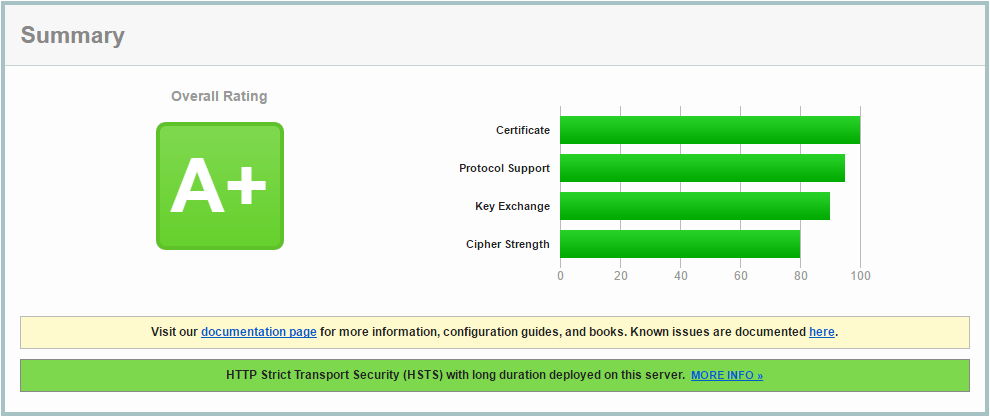
\includegraphics[width=0.9\textwidth]{res/evernote}
				\caption{Отчет для сайта evernote.com}
				\label{ris:evernote}
			\end{figure}
			
			\begin{itemize}
				\item Поддерживает все типы протоколов TLS;
				\item Поддерживает длительное форсированное защищенное соединение через 
				HTTPS.
			\end{itemize}
			
			В качестве домена из раздела Recent Worst был выбран домен 
			monabo.lemonde.fr.
			Отчет представлен на рисунке~\ref{ris:evernote}.
			
			\begin{figure}[h]
				\centering
				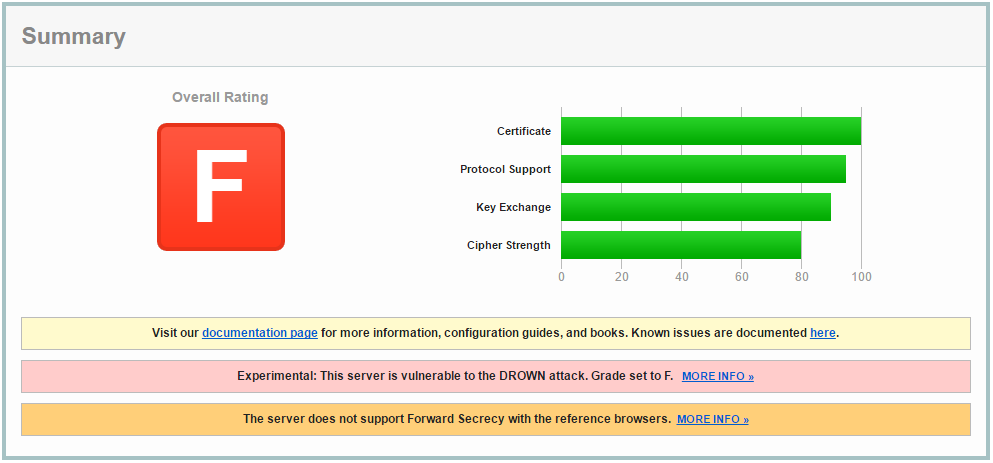
\includegraphics[width=0.9\textwidth]{res/monabo}
				\caption{Отчет для сайта monabo.lemonde.fr}
				\label{ris:monabo}
			\end{figure}
			
			\begin{itemize}
				\item Этот сервер подвержен DROWN атакам;
				\item Сервер не поддерживает Forward Security для браузеров.
			\end{itemize}
			
			Для самостоятельного анализа был выбран сервер habrahabr.ru.
			Результаты анализа приведены на рисунке~\ref{ris:habr}
			
			\begin{figure}[h]
				\centering
				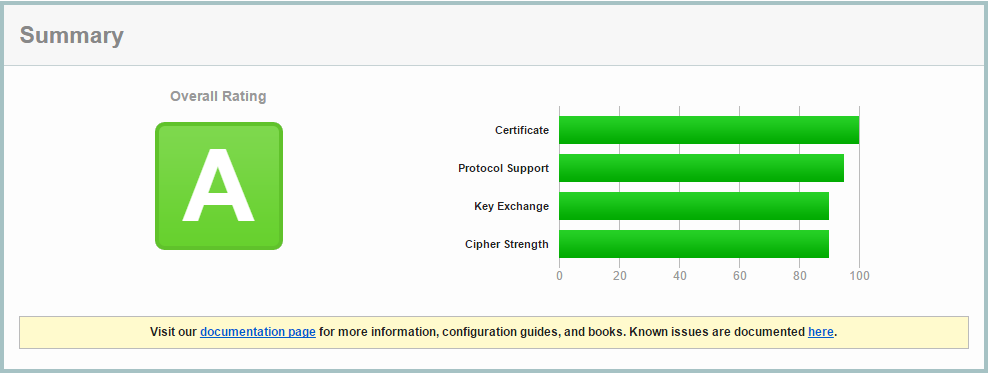
\includegraphics[width=0.9\textwidth]{res/habr}
				\caption{Отчет для сайта habrahabr.ru}
				\label{ris:habr}
			\end{figure}
			
			Как видно из рисунка~\ref{ris:habr}, сервис habrahabr.ru поддерживает все 
			типы протоколов TLS и не имеет проблем с безопасностью.
			
		\subsection{Расшифровка аббревиатур}
			Аббревиатуры представлены ниже:
			\begin{lstlisting}
TLS_ECDHE_RSA_WITH_AES_128_GCM_SHA256 (0xc02f)   ECDH secp256r1 (eq. 3072 bits 
RSA)   FS	128
TLS_ECDHE_RSA_WITH_AES_256_GCM_SHA384 (0xc030)   ECDH secp256r1 (eq. 3072 bits 
RSA)   FS	256
TLS_DHE_RSA_WITH_AES_128_GCM_SHA256 (0x9e)   DH 2048 bits   FS	128
TLS_DHE_RSA_WITH_AES_256_GCM_SHA384 (0x9f)   DH 2048 bits   FS	256
TLS_ECDHE_RSA_WITH_AES_128_CBC_SHA256 (0xc027)   ECDH secp256r1 (eq. 3072 bits 
RSA)   FS	128
TLS_ECDHE_RSA_WITH_AES_128_CBC_SHA (0xc013)   ECDH secp256r1 (eq. 3072 bits 
RSA)   FS	128
TLS_ECDHE_RSA_WITH_AES_256_CBC_SHA384 (0xc028)   ECDH secp256r1 (eq. 3072 bits 
RSA)   FS	256
TLS_ECDHE_RSA_WITH_AES_256_CBC_SHA (0xc014)   ECDH secp256r1 (eq. 3072 bits 
RSA)   FS	256
TLS_DHE_RSA_WITH_AES_128_CBC_SHA256 (0x67)   DH 2048 bits   FS	128
TLS_DHE_RSA_WITH_AES_128_CBC_SHA (0x33)   DH 2048 bits   FS	128
TLS_DHE_RSA_WITH_AES_256_CBC_SHA256 (0x6b)   DH 2048 bits   FS	256
TLS_DHE_RSA_WITH_AES_256_CBC_SHA (0x39)   DH 2048 bits   FS	256
TLS_RSA_WITH_AES_128_GCM_SHA256 (0x9c)	128
TLS_RSA_WITH_AES_256_GCM_SHA384 (0x9d)	256
TLS_RSA_WITH_AES_128_CBC_SHA (0x2f)	128
TLS_RSA_WITH_AES_256_CBC_SHA (0x35)	256
TLS_RSA_WITH_AES_256_CBC_SHA256 (0x3d)	256
TLS_RSA_WITH_AES_128_CBC_SHA256 (0x3c)	128
TLS_DHE_RSA_WITH_CAMELLIA_256_CBC_SHA (0x88)   DH 2048 bits   FS	256
TLS_RSA_WITH_CAMELLIA_256_CBC_SHA (0x84)	256
TLS_DHE_RSA_WITH_CAMELLIA_128_CBC_SHA (0x45)   DH 2048 bits   FS	128
TLS_RSA_WITH_CAMELLIA_128_CBC_SHA (0x41)	128
TLS_RSA_WITH_3DES_EDE_CBC_SHA (0xa)	112
TLS_ECDHE_RSA_WITH_3DES_EDE_CBC_SHA (0xc012)   ECDH secp256r1 (eq. 3072 bits 
RSA)   FS
			\end{lstlisting}
			
			Расшифровка аббревиатур:
			\begin{itemize}
				\item TLS\_ECDHE - алгоритм Диффи-Хэлмана на эллиптических кривых;
				\item RSA - алгоритм шифрования с открытым ключем;
				\item AES\_128 - алгоритм шифрования с длиной ключа в 128 бит;
				\item GCM и CBC - режимы блочного шифрования;
				\item SHA256 - хэш-функция с длиной ключа 256 бит.
			\end{itemize}
			
		\subsection{Описание позиций в разделе Protocol Details}
			Содержимое раздела Protocol Details представлено ниже:
			\begin{itemize}
				\item Проверка сертификата:
				\begin{lstlisting}
Secure Renegotiation	Supported
Secure Client-Initiated Renegotiation	No
Insecure Client-Initiated Renegotiation	No
				\end{lstlisting}
				
				\item Уязвимость к атакам Poodle, Bcast, Downgrade
				\begin{lstlisting}
BEAST attack	Not mitigated server-side (more info)   TLS 1.0: 0xc013
POODLE (SSLv3)	No, SSL 3 not supported (more info)
POODLE (TLS)	No (more info)
Downgrade attack prevention	Yes, TLS_FALLBACK_SCSV supported (more info)
				\end{lstlisting}
				
				\item Слабый алгоритм RC4 не используется
				\begin{lstlisting}
RC4	No
				\end{lstlisting}
				
				\item Сервер защищен от атак HeartBleed
				\begin{lstlisting}
Heartbeat (extension)	No
Heartbleed (vulnerability)	No (more info)
				\end{lstlisting}
				
				\item Совместимость Forward Security с браузерами
				\begin{lstlisting}
Forward Secrecy	Yes (with most browsers)   ROBUST (more info)
				\end{lstlisting}
				
				\item Наличие NPN (присутствует).
				В настоящее время используется для согласования использования SPDY в 
				качестве протокола прикладного уровня.
				\begin{lstlisting}
				NPN	Yes   http/1.1
				\end{lstlisting}
				
				\item Параметры сессии.
				\begin{lstlisting}
Session resumption (caching)	Yes
Session resumption (tickets)	Yes
				\end{lstlisting}
				
				\item Реализация HSTS.
				\begin{lstlisting}
Strict Transport Security (HSTS)	Yes   TOO SHORT (less than 180 days) 
max-age=900
HSTS Preloading	Not in: Chrome  Edge  Firefox  IE  Tor
				\end{lstlisting}
				
				\item Реализация HPKP (отсутствует).
				\begin{lstlisting}
Public Key Pinning (HPKP)	No
				\end{lstlisting}
				
				\item Совместимость с SSL2 (совместим).
				\begin{lstlisting}
SSL 2 handshake compatibility	Yes
				\end{lstlisting}
			\end{itemize}
		
		\subsection{Вывод о реализации SSL на выбранном домене}
			Исходя из отчета, сервис habrahabr.ru имеет хорошую конфигурацию: сервер 
			использует доверенный сертификат и защищен от основных типов атак.
			Так же сервис не использует устаревший алгоритм RC4, который является 
			уязвимым.
			Так же сервис имеет поддержку Forward Security для большинства браузеров.
			Исходя из этого, можно сделать вывод о том, что сервис хорошо защищен.
	
	\section{Выводы}
		В данной лабораторной работе были изучены возможности сервиса <<SLLLabs>>, 
		анализирующего качество защиты домена.
		Были разобраны отчеты, предоставляемые сервисом, а так же проанализирована 
		защита сервиса habrahabr.ru.
		Сервис позволяет увидеть защищенность домена от различных атак, а так же 
		список используемых протоколов.
\end{document}